% Scaled Dot-Product Attention — canonical anchored LTR-safe version
% \begin{LTR} prevents RTL mirroring from Polyglossia's global RTL context.
% every node/.style includes anchor=center so text sits exactly on each shape.
\begin{LTR}
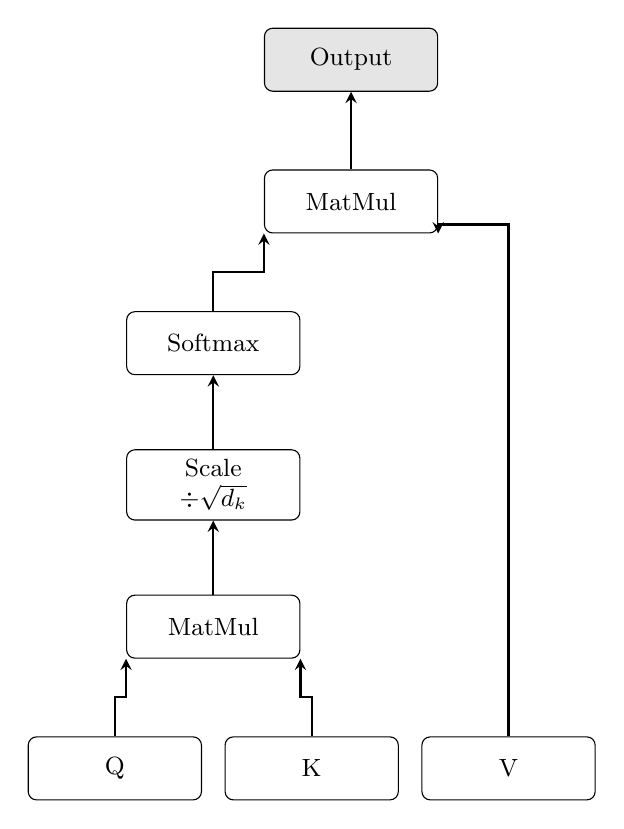
\begin{tikzpicture}[
    every node/.style={
        draw,
        rounded corners=3pt,
        minimum width=2.2cm,
        minimum height=0.8cm,
        align=center,
        anchor=center,
        font=\small
    },
    arrow/.style={->, >=stealth, thick}
]

% Input nodes — bottom row
\node (Q)       at (0,   0) {Q};
\node (K)       at (2.5, 0) {K};
\node (V)       at (5,   0) {V};

% Computation chain (left branch, 1.8 cm vertical spacing > 0.8 cm node height)
\node (matmul1) at (1.25, 1.8) {MatMul};
\node (scale)   at (1.25, 3.6) {Scale \\ \(\div\sqrt{d_k}\)};
\node (softmax) at (1.25, 5.4) {Softmax};

% Merge + output
\node           (matmul2) at (3.0, 7.2) {MatMul};
\node[fill=gray!20] (output)  at (3.0, 9.0) {Output};

% Q and K feed into first MatMul
\draw[arrow] (Q.north) -- ++(0,0.5) -| (matmul1.south west);
\draw[arrow] (K.north) -- ++(0,0.5) -| (matmul1.south east);

% Vertical computation chain
\draw[arrow] (matmul1.north) -- (scale.south);
\draw[arrow] (scale.north)   -- (softmax.south);

% Softmax and V feed into second MatMul
\draw[arrow] (softmax.north) -- ++(0,0.5) -| (matmul2.south west);
\draw[arrow] (V.north)       -- ++(0,6.5) -| (matmul2.south east);

% Final output
\draw[arrow] (matmul2.north) -- (output.south);

\end{tikzpicture}
\end{LTR}
